\section{提案手法}
本研究では、記号実行とファジングの解析手法を組み合わせることで、スケーラビリティと精度の両立を目指すSpectre gadget検出手法を提案する。記号実行とファジングにはそれぞれ利点と欠点が存在するが、これらを組み合わせることで、両者の欠点を補完し、スケーラビリティと精度を両立できるのではないかと考える。提案手法は、記号実行フェーズとファジングフェーズの2つのフェーズで構成され、それぞれのフェーズで検出されたgadgetを合わせて、最終的な検出結果として報告する。記号実行フェーズでは、ネストされた分岐予測を制限することで、投機的状態の探索範囲を縮小し、解析のスケーラビリティを向上させる。ファジングフェーズでは、記号実行フェーズで探索されなかった投機的な状態を集中的にテストすることで、記号実行で見逃されたgadgetを効率的に検出することを目指す。\par
以下では、記号実行フェーズとファジングフェーズのそれぞれについて、提案手法の詳細を説明する。

\subsection{記号実行フェーズ}
\subsubsection{ネストされた分岐予測の制限}
記号実行フェーズでは、ネストされた分岐予測を制限することでスケーラビリティの向上を図る。提案手法の記号実行フェーズがどのように投機実行をシミュレートするかについて、図\ref{MotivatingExample}の制御フローグラフの一部である図\ref{fig:SpecOrder_cfg}を用いて説明する。点線が分岐予測ミス、実線が通常の実行パスを表す。\par
まず、既存手法と同様に、解析が分岐\var{b1}に到達すると、投機実行のシミュレーションが開始され、以下の4つの状態に分岐する。\par

\begin{enumerate}
  \item 分岐\var{b1}の条件を満たし、Aに遷移した状態
  \item 分岐\var{b1}の条件を満たさず、Bに遷移した状態
  \item 分岐\var{b1}の条件を満たさず、分岐予測ミスによりAに遷移した状態
  \item 分岐\var{b1}の条件を満たし、分岐予測ミスによりBに遷移した状態
\end{enumerate}

これらのうち、3番目の状態のみが23行目の脆弱性を引き起こし、Spectre gadgetとして検出される。この状態から解析を進めていくと、次に分岐\var{b2}に遭遇する。既存手法では、ネストされた投機実行をシミュレートするため、\var{b2}でも分岐予測ミスを含めた4つの状態に分岐する。一方、提案手法ではネストされた分岐予測を制限し、\var{b2}における分岐予測ミスによる投機的な状態は探索しない。そのため、この状態において、以降は、投機ウィンドウの上限に達するか、直列化命令に遭遇するまで、正しい分岐方向の状態のみを探索し続ける。\par

その結果、11行目と14行目の脆弱性を引き起こすgadgetが見逃されてしまう。しかし、先述の通り、ネストされた分岐予測ミスにより引き起こされるされるgadgetは稀であるため、影響は少ないと考える。また、このようなネストされた分岐予測ミスにより到達する投機的な状態は、後述するファジングフェーズで探索を行うことで、False nagativeを最小限に抑え、精度を担保できると考える。\par

\begin{figure}[tb]
  \centering
  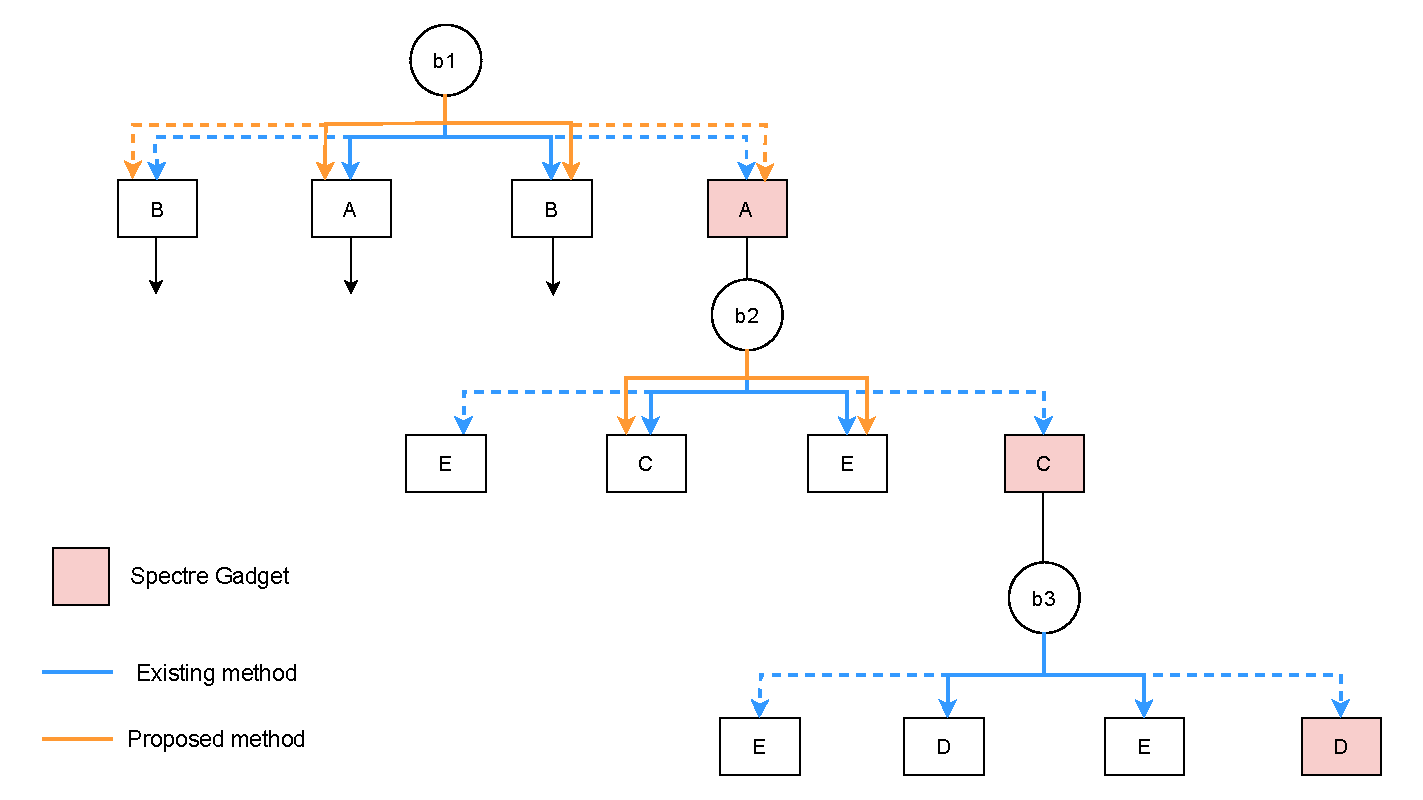
\includegraphics[width=\linewidth]{img/SpecOrder_cfg.drawio.pdf}
  \caption{ネストされた分岐予測ミスの制限}\label{fig:SpecOrder_cfg}
\end{figure}

\subsubsection{不要な分岐予測ミスの特定}
記号実行で探索されなかったネストされた分岐予測ミスにより到達する投機的な状態はファジングフェーズで探索を行う。この際、記号実行で探索した投機的な状態を再度、ファザーで探索するのは非効率的である。そこで、記号実行の過程で、分岐予測ミスをシミュレートしても、シミュレーションが終了するまでに別の分岐命令に到達できない分岐方向を特定する。その情報をファザーに提供し、それらの分岐方向への分岐予測ミスのシミュレーションを抑制することで、ファジングのスループットを向上させる。\par
図\ref{}に示すコード例を用いて具体的に説明する。


\subsubsection{目的状態までの実行トレースの取得}
\subsection{ファジングフェーズ}
\subsubsection{不要な分岐予測の抑止}
\subsubsection{スコアによるシードのスケジューリング}
